\documentclass[10pt,draftclsnofoot,onecolumn,letterpaper]{IEEEtran}
\usepackage[utf8]{inputenc}
\usepackage{blindtext}
\usepackage[english]{babel}
\usepackage[style=numeric,sorting=nty]{biblatex}
\usepackage{csquotes}
\usepackage{graphicx}
\usepackage{url}
\usepackage{setspace}

\addbibresource{mybib.bib}

\title{Technology Review: Mixed Reality For Infrastructure Maintenance}
\author{Team 20: Christopher C Cooper}
\date{November 2018}

\usepackage{geometry}
\geometry{textheight=9.5in, textwidth=7in}

% 1. Fill in these details
\def \CapstoneTeamName{		xRLucid}
\def \CapstoneTeamNumber{		20}
\def \GroupMemberOne{			Christopher Cooper}
\def \GroupMemberTwo{			Austin Liang}
\def \GroupMemberThree{			David Okubo}
\def \GroupMemberFour{			Jonathan Chen}
\def \GroupMemberFive{			Mingyu Zhang}
\def \CapstoneProjectName{		Mixed Reality for Infrastructure Maintenance}
\def \CapstoneSponsorCompany{	OSU School of Civil and Construction Engineering}
\def \CapstoneSponsorPerson{		Yelda Turkan}

% 2. Uncomment the appropriate line below so that the document type works
\def \DocType{	%	Problem Statement
				%Requirements Document
				Technology Review
				%Design Document
				%Progress Report
				}
			
\newcommand{\NameSigPair}[1]{\par
\makebox[2.75in][r]{#1} \hfil 	\makebox[3.25in]{\makebox[2.25in]{\hrulefill} \hfill		\makebox[.75in]{\hrulefill}}
\par\vspace{-12pt} \textit{\tiny\noindent
\makebox[2.75in]{} \hfil		\makebox[3.25in]{\makebox[2.25in][r]{Signature} \hfill	\makebox[.75in][r]{Date}}}}
% 3. If the document is not to be signed, uncomment the RENEWcommand below
\renewcommand{\NameSigPair}[1]{#1}

%%%%%%%%%%%%%%%%%%%%%%%%%%%%%%%%%%%%%%%
\begin{document}
\begin{titlepage}
    \pagenumbering{gobble}
    \begin{singlespace}
    	
\includegraphics[height=4cm]{coe_v_spot1}
        \hfill 
        % 4. If you have a logo, use this includegraphics command to put it on the coversheet.
        %\includegraphics[height=4cm]{CompanyLogo}   
        \par\vspace{.2in}
        \centering
        \scshape{
            \huge CS Capstone \DocType \par
            {\large November 9, 2018}\par
            \vspace{.5in}
            \textbf{\Huge\CapstoneProjectName}\par
            \vfill
            {\large Prepared for}\par
            \Huge \CapstoneSponsorCompany\par
            \vspace{5pt}
            {\Large\NameSigPair{\CapstoneSponsorPerson}\par}
            {\large Prepared by }\par
            Group\CapstoneTeamNumber\par
            % 5. comment out the line below this one if you do not wish to name your team
            \CapstoneTeamName\par 
            \vspace{5pt}
            {\Large
                \NameSigPair{\GroupMemberOne}\par
                %\NameSigPair{\GroupMemberTwo}\par
                %\NameSigPair{\GroupMemberThree}\par
                %\NameSigPair{\GroupMemberFour}\par
                %\NameSigPair{\GroupMemberFive}\par
            }
            \vspace{20pt}
        }

\begin{abstract}
Industrial maintenance and engineering have been looking to utilize Mixed Reality recently, creating a software to view Building Information Models in MR. With mixed reality, it is important to get a strong foundation of the user's experience through the hardware used. For display devices, Microsoft HoloLens serves the purpose well, but is overall too expensive and has a limited field of view while the newer MR headset, Magic Leap Pro improves the processing power and comfortability of the experience but is still too expensive for the common user. Mobile tablets provide a cheap and decent AR experience for wide spread adoption of the technology, making it the ideal choice for infrastructure engineers. Tracking of the user is the next important component of the hardware necessary for MR and the sensors typically seen in mobile phones, accelerometer, gyroscope, and magnetometer, are the best combination of accuracy and portability. GPS is far too inaccurate and the Antilatency system for tracking with IR has no release date. This puts the built-in sensors of the mobile device as the best option. Finally for user input, touch screens provide a simple and intuitive system that is not affected by typical environments of use. Voice recognition works well for navigating complex tasks, but works poorly in loud environments. The last input method was motion tracking with a controller. This input method does not provide enough difference from a touch screen when using a mobile tablet device, so it falls behind the standard touch screen. Therefore, the recommendation is to use a mobile tablet that supports ARCore, without the addition of peripherals for position tracking and user input.
\end{abstract}
\end{singlespace}
\end{titlepage}
\newpage
\pagenumbering{arabic}
\tableofcontents
\listoffigures
\listoftables
\newpage
\section{Introduction}
Mixed reality is an up and coming technology that seemingly has several companies interested. Mixed reality as a concept is the blending of computer generated objects and environments with the user's true surroundings. The idea is expanded by Microsoft to be a spectrum, settling between an Augmented Reality and Virtual Reality\cite{MRWhat}.
As a spectrum of content, mixed reality allows for a various quantities of digital elements displayed and various levels of interaction with those digital elements. This is why it requires high end hardware that can support the visualization and interaction of all components in an experience designed for MR.\par
\begin{figure}[ht]
    \centering
    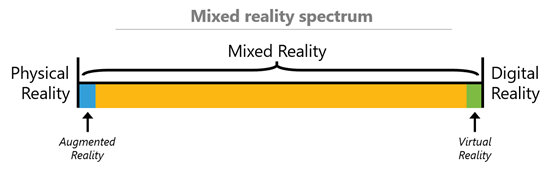
\includegraphics[width=0.75\textwidth]{mixed-reality-spectrum.png}
    \caption{Mixed Reality Spectrum\cite{MRWhat}}
    \label{fig:my_label}
\end{figure}
Industrial engineering and maintenance has begun looking into options for use of MR in its field, utilizing Building Information Models to visualize the project. Building Information Models are files containing a 3D model and all information of the project from the design phase to the demolition of the structure. With these models, visualization of maintenance information becomes possible for those in the field without access to large computers. This is the goal of the MR for Industrial Maintenance Project, to create a software that allows the easy visualization and modification of these models.\par

\section{Display Device for Mixed Reality}
Mixed reality is, by nature, a visual experience. The core of the experience is in seeing and interacting with computer graphics and real world objects simultaneously. In order to start, a user must be capable of seeing the computer generated graphics clearly, without compromising their visual understanding of their true surroundings.\par
\subsection{Microsoft HoloLens}
Microsoft HoloLens was one of the earliest products released specifically for mixed reality. The headset was originally launched as a developer kit to potential developers in March 2016. The mixed reality headset has a cost of \$3,000 for the developer edition that was released\cite{HL}. This edition is available to anyone with a Microsoft account.\par
The device overall is reasonably sized, weighing in at 1.2 lbs with a transparent lens going over the eyes and a band wrapping around the head\cite{HLspecs}. This weight is slightly heavier than a small iPad, which may in practice be a bit unwieldly as a headset. The headset has several sensors for gathering data from the real world including an inertial measurement unit, ambient light sensor, depth detecting camera, and four cameras to detect the environment\cite{HL}. These sensors working together, provide the information needed to project 3D models onto the environment convincingly. This is where the HoloLens is particularly interesting. The HoloLens with all the hardware packed into it, making it a headset not bound to a computer for processing power, displays true 3D computer generated models onto the environment\cite{HL}.\par
The headset is not all good news however. There is only a small, central area on the lenses that actually display the 3D models, which Microsoft says is to preserve the user's peripheral vision\cite{HLpromo}. This does make sense so far as being able to maintain awareness of surroundings, however it does mean that the mixed reality experience is not fully immersing.\par

\subsection{Magic Leap One}
Magic Leap One is a recently released contender in the AR/MR headset market. The headset is another self-contained device that does not require being hooked up to a computer\cite{MLO}. The website for the Magic Leap One, claims the device makes digital content contextually aware of the environment using the sensors (exactly what sensors these are, the company does not specify)\cite{MLOpromo}.\par
In most respects, the Magic Leap One is a slightly cheaper HoloLens, with the Magic Leap One being priced at \$2,295\cite{MLOpromo}. But there are things that differentiate it. The most obvious at first glance is the belt pack containing most of the processing hardware for the Magic Leap One, taking some of the hardware away from the headset itself\cite{MLOpromo}. This allows the Magic Leap One to maintain a small frame while having 128GB of storage and 8GB of RAM\cite{MLOpromo}. One of the more impressive features of the Magic Leap One, is the display. Magic Leap One is meant to project the image directly on the retina, allowing computer generated objects to be focused on in the same way a person's eyes ordinarily do\cite{MLO}. The other improvement that Magic Leap has made, is that Magic Leap One can block real objects with the computer generated objects, preserving the immersion of the user\cite{MLO}. Although the Magic Leap One has many noteworthy features, the field of view for the device is still very limiting\cite{MLO}. For the ease of use with the Magic Leap One, there is an SDK for development that can integrate with the Unity and Unreal engines\cite{MLSDK}.\par

\subsection{Mobile Tablet}
Mobile tablets such as iOS and Android, along with mobile phones, are not inherently devices meant for AR, MR, or VR experiences. They do, however, have many sensors that can help them be used in these ways. For the context of AR/MR there are two SDKs available (one for Android and the other for iOS) that assist in making these unique experiences. The Android SDK is called ARCore, while the iOS SDK is called ARKit. Both of these SDKs are created by the respective mobile OS developers. Mobile phones and tablets, use a collection of sensors including accelerometer, gyroscope, and magnetometer to determine the position and orientation of the device in three-dimensional space\cite{PhoneSense}. This provides a foundation for a developer to create an AR experience. To assist them, Apple and Google created their SDKs. Both SDK offerings assist the developer by providing tools for motion tracking and scene processing from the device's camera\cite{ARKdoc}\cite{ARCdoc}.\par
The main appeal to this device is not the robust hardware for AR/MR experiences, but the much cheaper price. A tablet is priced at hundreds of dollars as opposed to thousands, making it a more widely attainable platform to launch AR/MR applications for the near future. This project will push the AR capabilities of the device to the limit, meaning any improvements would most likely require a new platform.\par

\subsection{Comparison}

Despite the advantages of a hands free device such as the HoloLens and Magic Leap One, the price causes these devices to not be readily available enough for any reliance. This, coupled with large designs that could cause concern for long use and limited number of available development tools on the market make these two displays not worth the large investment at this time. Moreover, the project does not necessitate many of the mixed reality features that make the head-mounted displays enticing and the AR of a mobile device will be sufficient.\par

\begin{table}[ht]
\begin{center}
\caption{Comparison of Display Device Features}
\label{table:1}
 \begin{tabular}{|p{3cm}|p{1cm}|p{2cm}|p{5cm}|p{2cm}|} 
 \hline
 Device & Price & Field of View & Available Development Tools & Size \\ [0.5ex] 
 \hline\hline
 Microsoft HoloLens & \$3,000 & Small & Limited & Large \\ 
 \hline
 Magic Leap One & \$2,295 & Small & Limited & Small \\
 \hline
 Mobile Tablet/Phone & \$329 & Medium & Numerous & Large \\
 \hline
\end{tabular}
\end{center}
\end{table}

\section{Acquiring 3D Position of the User}
For mixed reality to work correctly as a convincing experience, the user must see a reasonable translation of the computer graphic elements according to their own motions. This brings forth the need to accurately track the position of the user to determine their position within the 3D coordinates of the computer graphics scene.\par
\subsection{Sensors: Accelerometer, Gyroscope, Magnetometer}
The accelerometer, gyroscope, and magnetometer are most likely known to the average person from their use in smart phones. These sensors work together, creating an image of the device's position and orientation in the real world. This is an included part of mobile devices as well as the head-mounted displays.\par
The accelerometer is a sensor that measures both vibration and acceleration. This is accomplished by the acceleration causing a mass in the sensor to press on a material that then produces an electric charge with a magnitude of the force applied to it. This is the basic principle of the accelerometer\cite{Accel}. That is all an accelerometer measures, acceleration along an axis. This is not enough to get a good idea of the motion that a device has been subjected to, but it is a start.\par
The next sensor is the gyroscope. This sensor is simple in that it detects orientation by using Earth's gravitational pull to always know where down is\cite{Gyro}. This can be combined with the accelerometer, creating an image of the orientation of the device during the acceleration detected by the accelerometer (if there is one).\par
The final sensor is the magnetometer. The magnetometer is a small sensor that senses the magnetic field of Earth to determine which direction is North and relays this to the device through varying the voltage output. This sensor is the final sensor of three that are commonly used by phones to determine the device's position and orientation\cite{PhoneSense}.\par
These sensors can only determine the position of the device and relies completely on the device app correctly using the information to calculate that position, but these sensors are cheap and widely available to obtain for use in many devices. In addition, even with all sensors working together, the user only has three degrees of freedom. These degrees of freedom are the orientation of the user and thus a user must stand still for an AR experience. This problem is fixed only by using ARCore, an SDK by Google that gives six degrees of freedom to mobile devices\cite{AR6dof}. However, this SDK only works on selected devices\cite{ARdev}.

\subsection{GPS: Global Positioning System}
GPS is a system consisting of 30 satellites orbiting the Earth, ground stations, and receivers. The satellites are useful since we know where they are at any time, while the ground stations are used to ensure they are actually where they are supposed to be. Receivers then communicate with the satellites to determine how far away four or more of them are from itself. This gives a general idea of where the user is, but only high-end receivers can calculate the position within a few inches\cite{GPS}. The typical smart phone is only accurate within approximately 16 feet under good conditions\cite{GPSacc}. This is far from a good accuracy to use within an AR/MR experience for the user's position. Though it is too inaccurate for most uses, it can be sufficient for automatic loading of an experience based on location within a town. These receivers can price in the \$20-\$50 range so the are reasonably priced and readily available as an add-on for tablets without built-in receivers.

\subsection{External Sensors: Inside Out Tracking}
Motion capture typically consists of several cameras and a set of markers on the user's body to create detailed 3D motions for use in films and games\cite{MoCap}. This is similar to the camera setup used for the VR headsets HTC Vive and Oculus Rift. The motion capture equipment is typically expensive, but there was a proposed solution in 2014 that would make use of a human pose database to reconstruct the pose even if information from the cameras were missing\cite{MoCap}. This approach, gathering information about a user's pose, is overkill for a simple MR application, and so a simplified solution would be more appropriate. This leads to Antilatency.\par

Antilatency is a start-up that is creating a positional tracking solution for mobile VR, virtual reality. Though it is for VR, the tracking elements of VR are the same as for MR. This allows the solution to be utilized, even though it is intended for head mounted displays. The tracker is device agnostic, seemingly as long as the device has a data port similar to that of a phone (microUSB). The device then tracks strips with IR markers called a reference bar to create the tracking area. This allows an individual to buy more reference bar to expand the tracking area. The device is priced at \$99 per tracker and reference bar combo. The problem with this solution though is that it is not released yet. The company claims it is close to manufacture but as of right now, there is no device to receive even with a purchase. They are allowing customers to preorder the device, but a release date has not even been mentioned\cite{AL}.\par

\subsection{Comparison}

With the limited detection of GPS, there are only two real options for positional tracking. The accelerometer and gyroscope are already included in many AR devices, making them the cheapest solution, while also allowing for accurate tracking even though it is only three degrees of freedom. The Antilatency sensor is an appealing option that would be ideal due to its ability to work with many mobile devices, accurate tracking, and ease of scaling the tracking area. It is not ideal, however, because it is not released and has no expected release window. This makes the standard sensors of mobile devices the best choice for the near future, with specific device requirements to the software, as the six degrees of freedom provided by ARCore is needed for MR.\par

\begin{table}[ht]
\begin{center}
\caption{Comparison of User Tracking Device Features}
\label{table:2}
 \begin{tabular}{|p{3cm}|p{2cm}|p{3cm}|p{4cm}|p{3cm}|} 
 \hline
 Device & Price & Degrees of Freedom & Detect Small Motions & Tracking Area Size \\ [0.5ex] 
 \hline\hline
 Mobile Sensors & Included & 3 (6 with ARCore) & Yes & Not Limited \\ 
 \hline
 GPS & \$20-\$50 & 3 (translation) & No & Not Limited \\
 \hline
 Antilatency & \$100 & 6 & Yes & Limited by Tracking Strip Quantity \\
 \hline
\end{tabular}
\end{center}
\end{table}

\section{User Input Methods of Mixed Reality}
The final core component of a mixed reality experience is the user interaction with the computer generated objects. In this context, only the viability of hardware and implementation toolkits will be considered. This implies that the benefit of menu traversal, providing numerical data, and other elements related to the user's experience with the user interface will not be considered here. The three components that will be considered are: the viability of how accurately and reliably a user's input is recognized and recorded by the corresponding method of input, price, and the variety of input types it can handle.\par

\subsection{Touch Screen}
Touch screens are becoming more and more common with tablets, phones, and touch screen computers. This is due to the ease of use for these input devices. There is the small problem that touch screens provide no feedback to the user inherently, so this leads to potential error and inefficiency in completing a task\cite{TouchScreen}. The other part about touch screens is the size. The size of the screen has an impact on how well a user can perform a given task. According to a study performed by Anthony Jennings, Spencer Ryser and Frank Drews from the University of Utah, a tablet sized touch screen (7" diagonal) was slower but less effort was needed for tasks when compared to a phone screen (4.3" diagonal)\cite{TouchScreen}. This places an important task when deciding an interface for a user. Whether ease of use, or speed is more important for your application. For the project currently in question, accuracy of inputs is more important than speed. As such, a larger screen mobile device would be chosen.\par
The touch screen allows for any input that can be displayed on the screen as if being selected with a computer mouse. This combined with some gestures, such as scrolling, allows for nearly any input task to be accomplished.\par

\subsection{Hand Tracking}
Hand tracking is somewhat a recent input method, with early, well-known successes being the Nintendo Wii. Now, there are attempts to make mobile motion controllers. This is being done by a company called Finch Technologies that is creating a motion control solution for mobile devices called FinchDash. These controllers use the same sensors that are in mobile phones to track input with three degrees of freedom. This allows for gestures and several other inputs using a track pad and trigger in addition to the motion sensing. The controllers are paired with the smart phone using Bluetooth. This interface enables the controllers to be used with any iOS or Android device, making it viable for a wide range of products. The SDK is capable of integration with Unity and Unreal Engines, providing ease of development for applications with real-time application\cite{FD}.\par
The product seems to be well designed and has a low price tag of 69 dollars, but it limits some important input for the current project. With the use of Building Information Models there is a high quantity of text and numerical data to be viewed and potentially added/modified. While this is not impossible or even difficult for motion controls, it is more tedious then typing on a touch screen or speaking input. Since the controllers do not provide any significant motion control, such as having six degrees of freedom, there is not enough benefit to use the controller over other input devices. The motion controls would simply become gestures for the user to learn or a pointing device, which would hardly be a departure from pointing on a touch screen.

\subsection{Voice Commands}
Voice controlled devices are becoming more popular in recent years. Early on was the introduction of Siri to the iPhone, followed by Google's own voice-activated assistant. Then came the two home assistants, Amazon's Alexa and Google Home. The appeal of voice input for controlling certain tasks is the ability for users to avoid multiple menus and give one command for even a complex task. The major problem with utilizing voice commands as an input method is the reduction in reliability when in an environment with a high quantity of background noise\cite{MRInput}. This means that voice commands go down significantly in efficiency if the application is expected to be used outside of the privacy of the home. Voice recognition is also completely reliant on a decent microphone being available to capture the user's voice clearly enough for the software to determine the command given. The MR project for infrastructure maintenance does not have a high quantity of nested commands and is intended to be used outdoors near structures such as bridges and tunnels, therefore, the application would not efficiently make use of voice commands. This eliminates the need for consideration of an external microphone as opposed to the built-in option.

\subsection{Comparison}

Voice commands would not be efficient nor reliable in the project as nested menus will not even be included and noisy environments will be common. The FinchDash controller provides good input at a reasonable price, however the controller does not enhance the inputs available for the touch screen. Without providing anything new, the controller is wasted when the touch enabled device is in the hands of the user instead of on a head mount. User in the field would be best served by using the touch screen of the device exclusively.

\begin{table}[ht]
\begin{center}
\caption{Comparison of User Input Device Features}
\label{table:3}
 \begin{tabular}{|p{2cm}|p{3cm}|p{3cm}|p{3cm}|} 
 \hline
 Device & Price & Reliability & Input Variety \\ [0.5ex] 
 \hline\hline
 Touch Screens & Included for tablet & good in all environments & Menus, gestures, text \\ 
 \hline
 FinchDash & \$69 & good in all environments & Menus, gestures, text \\
 \hline
 Microphone & Included for tablet & Bad in noisy environments & Nested menus, text \\
 \hline
\end{tabular}
\end{center}
\end{table}

\section{Conclusion}
Mixed reality is still in its infancy, and with that, many design decisions regarding the best methods of display, tracking, and user input are still fluctuating. With the release of MR dedicated headsets such as the Microsoft HoloLens and Magic Leap One, there are now hands-free devices for enjoying AR/MR applications but are far too expensive for wide spread adoption. Tablets, on the other hand, are cheap and can provide a decent AR experience to its users and is the suggested method for now. Tracking of a user's position in 3D space comes down to two options: the portability of sensors commonly seen in phones, or the accuracy of inside out tracking. Inside out tracking does not currently have a viable solution for mobile devices that is currently available for purchase so the built-in sensors will have to make due. Finally with input, there are three great input methods in touch screen, motion, and voice recognition that ultimately comes down to what tasks you wish the user to be able to perform and where the app will be most used. The touch screen comes out ahead as the motion controls add nothing new when the touch screen device is in the hands of the user, and voice commands are unreliable in noisy environments such as a construction area. The recommendation is to use a mobile tablet that is supported by ARCore as is, with no external peripherals modifying it.

\newpage
\printbibliography
\end{document}
